% !TeX spellcheck = en_US

% Grab the package from https://github.com/PetteriAimonen/latex-datasheet-template
\documentclass{datasheet}

\usepackage{graphicx}
\usepackage{nameref}
\usepackage{soul}

\usepackage{tikz}
\usetikzlibrary{matrix,positioning,arrows,fit,calc}
% Fuckin TikZ magic; https://tex.stackexchange.com/a/653533
\tikzset{tight matrix/.style={every outer matrix/.append style={inner sep=+0pt}}}

\usepackage[table]{xcolor}
\newcolumntype{s}{>{\columncolor[HTML]{eeeeee}} l}

\newcommand{\iis}{I$^2$S}
\newcommand{\al}{AXI4-Lite}
\newcommand{\regs}[4]{\begin{tabularx}{\textwidth}{|s|*{8}{X|}}
		\hline
		Bit   & 31 & 30 & 29 & 28 & 27 & 26 & 25 & 24\\\hline
		Value & #1\\\hline\hline
		Bit   & 23 & 22 & 21 & 20 & 19 & 18 & 17 & 16\\\hline
		Value & #2\\\hline\hline
		Bit   & 15 & 14 & 13 & 12 & 11 & 10 &  9 &  8\\\hline
		Value & #3\\\hline\hline
		Bit   &  7 &  6 &  5 &  4 &  3 &  2 &  1 &  0\\\hline
		Value & #4\\\hline
\end{tabularx}}
\newcommand{\rzeroes}[1]{\multicolumn{#1}{c|}{0}}
\newcommand{\note}[1]{\colorbox[HTML]{eeeeff}{
		\begin{minipage}
			{\textwidth}{\Large\bfseries Note:} #1
		\end{minipage}
}}
\newcommand{\textoverline}[1]{$\overline{\mbox{#1}}$}

\title{CBI980AL}
\subtitle{\al\ Audio Interface}
\author{Bence Csókás}
\revision{Preliminary}
\companylogo{\Huge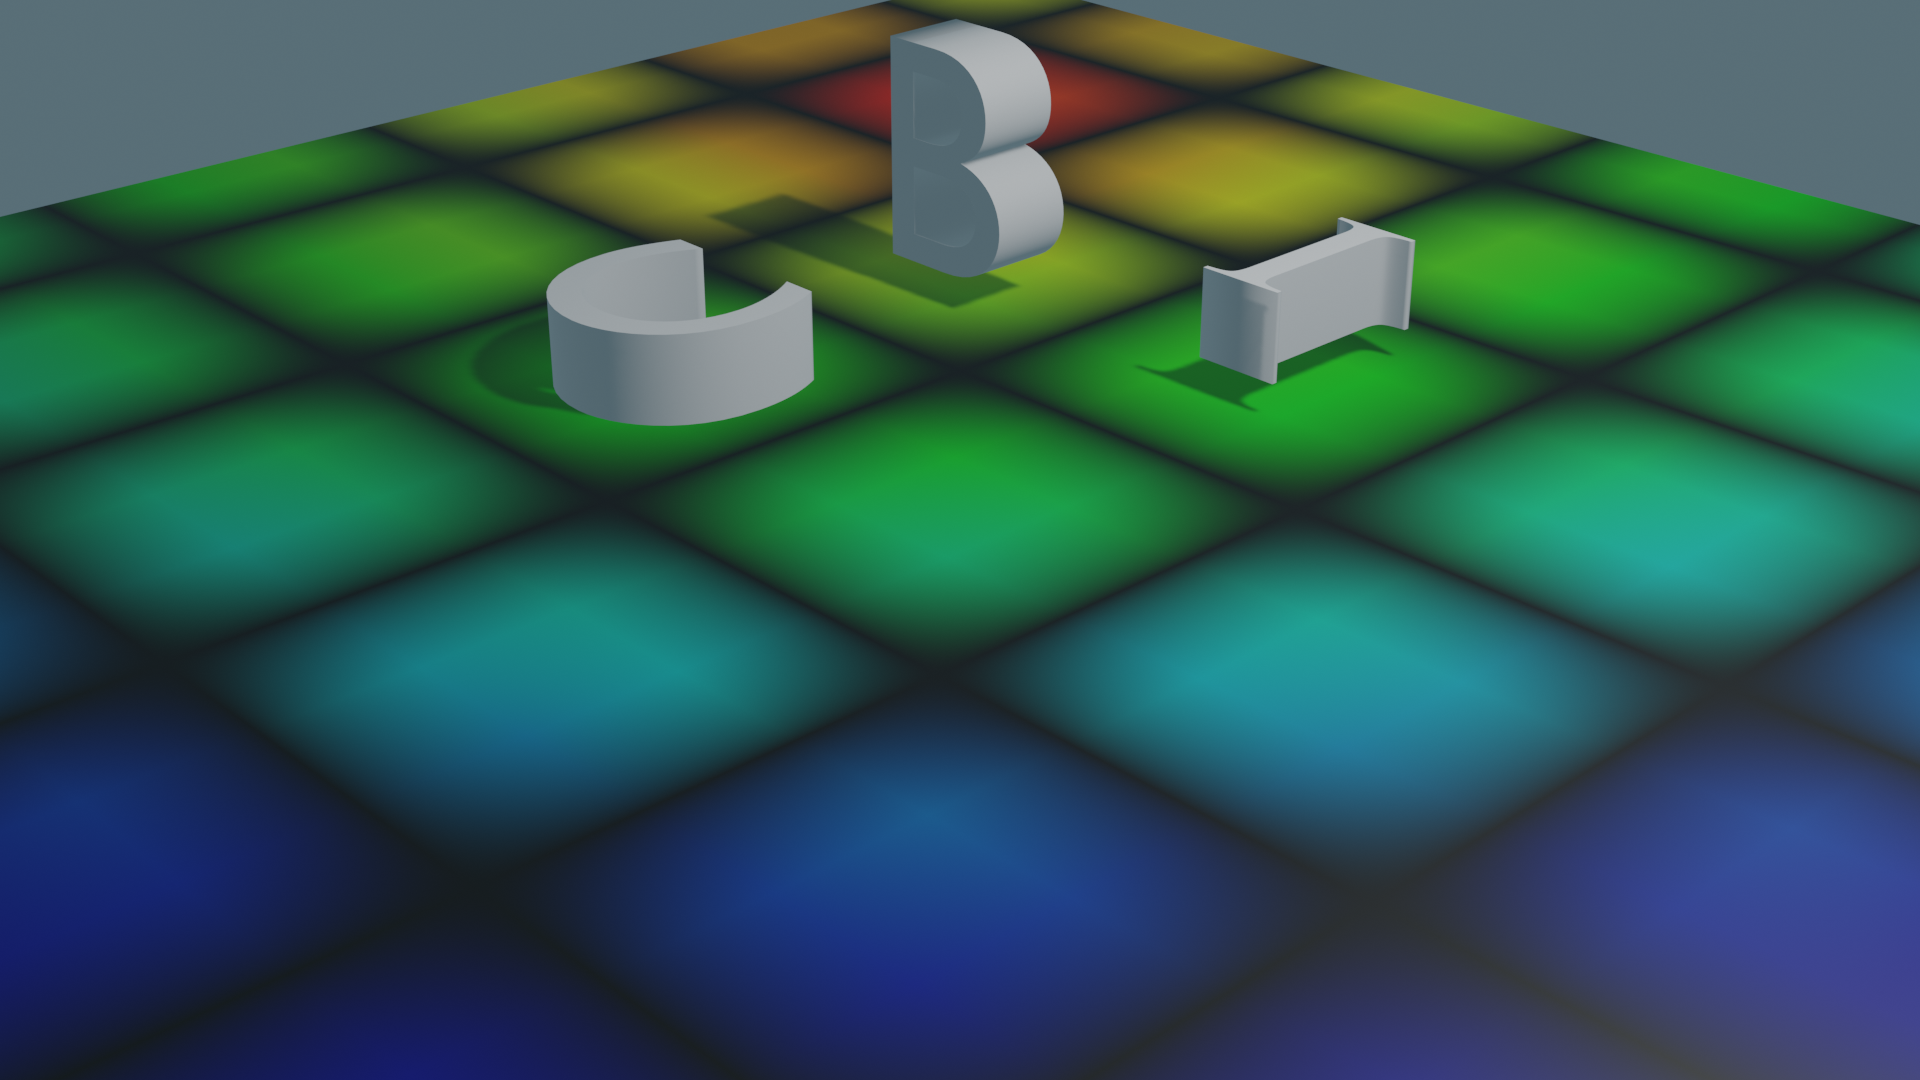
\includegraphics[width=3em]{cbilogo} CBI Semi}

\begin{document}
	\maketitle

	\section{Overview}
	AMBA \al\cite{a4l-spec}-controlled digital stereo audio input/output device with \iis\cite{i2s-spec} master interface

	\section{Features}
	\begin{itemize}
		\item 32-bit \al\ control and data interface with 8 registers
		\item 2 two-way channels with built-in data FIFO for stereo audio RX/TX
		%\item Configurable \iis\ line format
		\item FIFO overrun/underrun detection for \iis\ side
		\item Interrupt capability for all FIFO status flags
	\end{itemize}

	\vfill\break

	\begin{center}
		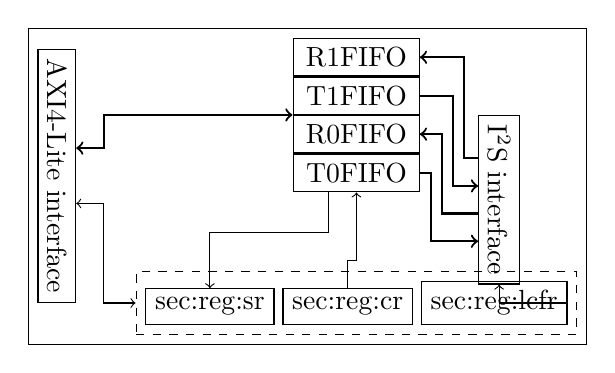
\begin{tikzpicture}
		\node[draw,rectangle,rotate=-90] (AXI) {\al\ interface};
		%\coordinate[right=of AXI](cMain);
		% Registers
		\matrix (mRegs) [matrix of nodes,right=of AXI,nodes={draw,rectangle,solid},column sep=0.1cm,draw,dashed,rectangle]{
		\nameref{sec:reg:sr} & \nameref{sec:reg:cr} & \nameref{sec:reg:lcfr}\\
		};

		%FIFOs
		\matrix (mFifos) [matrix of nodes,above=of mRegs,nodes={draw,rectangle,solid,text width=9ex,align=center},tight matrix]{
			R1FIFO\\
			T1FIFO\\
			R0FIFO\\
			T0FIFO\\
		};

		\node[draw,rectangle,rotate=-90,right=of mFifos] (I2S) {\iis\ interface};

		\node[draw,rectangle,fit=(AXI)(mRegs)(mFifos)(I2S)] (IC) {};

		\path[<->,draw]       ($(AXI.north)+(0,-1em)$) -- ++(1em,0) |- (mRegs.west);
			\path[<->,draw,thick] (AXI.north) +(0,1em)  -- ++(1em,1em) |- (mFifos.west);

		\path[<-,draw,thick]  (mFifos-1-1.east) -- +(16pt,0) |- ($(I2S.south)+(0,1.5em)$);
		\path[->,draw,thick]  (mFifos-2-1.east) -- +(12pt,0) |- ($(I2S.south)+(0,.5em)$);
		\path[<-,draw,thick]  (mFifos-3-1.east) --  +(8pt,0) |- ($(I2S.south)-(0,.5em)$);
		\path[->,draw,thick]  (mFifos-4-1.east) --  +(4pt,0) |- ($(I2S.south)-(0,1.5em)$);
		\path[->,draw]        (mRegs-1-3.east)  -| (I2S.east);
		\path[->,draw]        (mRegs-1-2.north) -- ++(0,1em) -| (mFifos.south);
		\path[<-,draw]        (mRegs-1-1.north) -- ++(0,2em) -| ($(mFifos.south)-(1em,0)$);
		\end{tikzpicture}
	\end{center}

	\onecolumn

	\section{Register map}
	\begin{minipage}{\textwidth}
		\begin{tabular}{|l|l|l|l|l|}
			\hline
			\textbf{Word Offset} & \textbf{Byte Offset} & \textbf{Register} & \textbf{Long Name} & \textbf{Access\footnote{RO=Read Only, RW=Read/Write, WO=Write Only}}\\\hline
			0 & 0000 & \nameref{sec:reg:cvr} & Chip ID/Version Register & RO\\\hline
			1 & 0004 & \nameref{sec:reg:sr} & Status Register & RO\\\hline
			2 & 0008 & \nameref{sec:reg:cr} & Control Register & RW\\\hline
			3 & 000C & \nameref{sec:reg:lcfr} & Line Coding Format Register & RW\\\hline
			4 & 0010 & \nameref{sec:reg:dout1r} & Data Output Channel \#1 Register & WO\\\hline
			5 & 0014 & \nameref{sec:reg:dout0r} & Data Output Channel \#0 Register & WO\\\hline
			6 & 0018 & \nameref{sec:reg:din1r} & Data Input Channel \#1 Register & RO\\\hline
			7 & 001C & \nameref{sec:reg:din0r} & Data Input Channel \#0 Register & RO\\\hline
		\end{tabular}
	\end{minipage}
	Violating access type (i.e. trying to write a RO register), or trying to write $<32$ bits at a time will result in a SLVERR. Writing an out-of-range or otherwise invalid value to a register will return OKAY, but the invalid portion of the write will not take effect (i.e. writing unallocated/constant bits in a register will be discarded, but the rest of the register will be updated).

	\subsection{CVR}\label{sec:reg:cvr}
	The CVR holds the chip's identifier, which, for the part covered by this document, is always \texttt{0xcb199800}

	\subsection{SR}\label{sec:reg:sr}
	SR holds the FIFO's status flags, as well as a flag indicating readiness after reset.

	\regs
		{Init & \rzeroes{7}}
		{\rzeroes{4} & RXOVF$_1$ & TXUNF$_1$ & RXOVF$_0$ & TXUNF$_0$}
		{RXNE$_1$ & RXF$_1$ & TXNF$_1$ & TXE$_1$ & RXNE$_0$ & RXF$_0$ & TXNF$_0$ & TXE$_0$}
		{\rzeroes{8}}

	\begin{itemize}
		\item Init: 0 after reset, 1 when the \iis\ interface is ready to send data
		\item RXOVF$_n$: $n$-th channel RX FIFO overflowed
		\item TXOVF$_n$: $n$-th channel TX FIFO underflowed
		\item RXF$_n$: $n$-th channel RX FIFO full
		\item TXNF$_n$: $n$-th channel TX FIFO not full
		\item TXE$_n$: $n$-th channel TX FIFO empty
		\item RXNE$_n$: $n$-th channel RX FIFO not empty
	\end{itemize}

	\subsection{CR}\label{sec:reg:cr}
	CR contains interrupt enable, transmit and receive enable bits, as well as the interrupt flag and a soft reset bit.

	\regs
		{\rzeroes{8}}
		{\rzeroes{4} & \multicolumn{4}{c|}{IE$_H$}}
		{\multicolumn{8}{c|}{IE$_L$}}
		{\rzeroes{2} & RXEN$_1$ & TXEN$_1$ & RXEN$_0$ & TXEN$_0$ & IF/INTc & RST}

	\begin{itemize}
		\item IE$_H$, IE$_L$: Interrupt Enable bits, the layout follows the corresponding bits in \nameref{sec:reg:sr}
		\item RXEN$_n$: $n$-th channel RX enable
		\item TXEN$_n$: $n$-th channel TX enable
		\item IF/INTc: Interrupt Flag, writing a 1 here clears previously latched RXOVF$_n$ and TXUNF$_n$ bits
		\item RST: Writing a 1 here performs a soft reset of the device; in this case, other bits will not take effect
	\end{itemize}

	\note{INTc will not necessarily clear the interrupt condition; namely, it will not clear RXF$_n$, TXNF$_n$, TXE$_n$, RXNE$_n$ (these stay active so long as the condition exists), nor will it clear RXOVF$_n$ and TXUNF$_n$ on the same clock cycle an over- or underflow occurs.}

	All flags in CR have a value of 0 after reset.

	\subsection{LCFR}\label{sec:reg:lcfr}
	This register \st{does nothing} sets the line coding format of the \iis\ interface.

	\regs
		{\rzeroes{5} & \multicolumn{3}{c|}{MCLK$_{rate}$}}
		{\rzeroes{5} & \multicolumn{3}{c|}{SCLK$_{rate}$}}
		{\rzeroes{5} & \multicolumn{3}{c|}{\#octets}}
		{\rzeroes{6} & R$_{just}$ & LSB$_{first}$}

	\begin{itemize}
		\item MCLK$_{rate}$: Division factor for MCLK, see \nameref{sec:clk:mclk}
		\item \#octets: Number of octets per sample to be transmitted, minus one. A value of 0 means 8 bits/sample, 1 means 16 bit, 2 means 24 bit and 3 means 32 bit
		\item R$_{just}$: In the case of the 24-bit format, specify alignment within the 32-bit-slot frame. 0 means left-justified (valid data towards the MSB), 1 means right-justified (valid data towards the LSB)
		\item LSB$_{first}$: Whether to transmit the Least Significant Bit (LSB) first or last. 0 means MSB first, LSB last, 1 means LSB first, MSB last
	\end{itemize}
	\note{According to the \iis\ specification\cite{i2s-spec}, data should be MSB first, and -- if justification is needed, -- left-justified, that is, LSB$_{first}$ and R$_{just}$ should both be 0 (their reset value). These options are there mostly for connecting to non-compliant devices.}

	The reset values for the fields in LCFR are:
	\begin{itemize}
		\item MCLK$_{rate}$: 0, meaning a clock division of 2
		\item \#octets: 2, meaning 24-bit mode
		\item R$_{just}$: 0, meaning left-justified
		\item LSB$_{first}$: 0, meaning MSB transmitted first, LSB last (standard \iis\ operation)
	\end{itemize}

	\subsection{Data registers}
	These 32-bit registers act as the datapath for the audio stream. Reading/writing these registers dequeues/enqueues words from/to the respective FIFOs. In cases where the data to be ent is less than 32 bits, the valid data will occupy the top bits of the register (that is, the input data is expected to be left-justified).

	\subsubsection{DOUT1R}\label{sec:reg:dout1r}
	TX Data Out for channel \#1.

	\subsubsection{DOUT0R}\label{sec:reg:dout0r}
	TX Data Out for channel \#0.

	\subsubsection{DIN1R}\label{sec:reg:din1r}
	RX Data In for channel \#1.

	\subsubsection{DIN0R}\label{sec:reg:din0r}
	RX Data In for channel \#0.

	\section{Clocks}\label{sec:clk}
	CBI980 is an \iis\ controller, as per chapter 3 of the specification\cite{i2s-spec}. The document mandates the presence of two 50\% duty cycle clock signals, both generated by the controller:
	\begin{itemize}
		\item \nameref{sec:clk:sclk} (Serial Clock): it times the data transmission
		\item \nameref{sec:clk:lrclk} (\textoverline{Left}/Right Clock)\footnote{Called WS (Word Select) by the specification, also sometimes called FS (Frame Sync)}: it specifies the sample rate ($f_S$)
	\end{itemize}
	On top of that, CBI980 also generates the following optional clock:
	\begin{itemize}
		\item \nameref{sec:clk:mclk} (Master Clock): it is used by the external \iis\ codec as a reference
	\end{itemize}

	All of the clocks specified here are synthesized from the \al\ clock (ACLK), with a power-of-two division.

	\subsection{SCLK}\label{sec:clk:sclk}
	SCLK is used for synchronizing the data I/O: new bits are to be sent by the transmitter at its falling edge, and sampled at the receiver on its rising edge.

	Internally, SCLK is obtained from ACLK by a frequency division factor of $2^{SCLK_{rate}+1}$, with \textit{SCLK$_{rate}$} being specified in \nameref{sec:reg:lcfr}.

	\subsection{LRCLK}\label{sec:clk:lrclk}
	LRCLK, on top of specifying the sample rate for the codec, also acts as a channel selector: on the low half-cycle, data for channel \#0 is shifted out/in, on the high half-cycle, channel \#1's transaction is performed.

	LRCLK is synthesized so that it has a frequency of $f_{LRCLK}\geq8\cdot\#octets\cdot f_{SCLK}$, while maintaining that $f_{LRCLK}=f_{ACLK}\cdot2^{-N}$ for some $N$ (the smallest such $N$ that satisfies the first requirement).

	\subsection{MCLK}\label{sec:clk:mclk}
	MCLK is needed by some codecs for a frequency reference base. Its typical frequency is equal to $256\cdot f_S$. Consult the datasheet of your codec to find the precise value/expected frequency range for your device.

	Internally, MCLK is obtained from ACLK by a frequency division factor of $2^{MCLK_{rate}+1}$, with \textit{MCLK$_{rate}$} being specified in \nameref{sec:reg:lcfr}.

	\pagebreak

	\begin{thebibliography}{9}
		\bibitem{a4l-spec}
		ARM: AMBA \al\ Interface Specification\\
		\url{https://developer.arm.com/documentation/ihi0022/e/AMBA-AXI4-Lite-Interface-Specification}
		\bibitem{i2s-spec}
		NXP Semiconductors: \iis\ bus specification, Rev. 3.0 (2022-02-17)\\
		\url{https://www.nxp.com/docs/en/user-manual/UM11732.pdf}
	\end{thebibliography}
\end{document}